\documentclass[10pt, aspectratio=169]{beamer}

\usetheme[progressbar=frametitle, sectionpage=progressbar, subsectionpage=progressbar, numbering=fraction, block=fill]{metropolis}

\definecolor{mLightBrown}{HTML}{4D4D4D}
\definecolor{mMediumBrown}{HTML}{2C2C2A}
\definecolor{mDarkBrown}{HTML}{1A1A19}
\definecolor{mDarkTeal}{HTML}{0F6E56}
\definecolor{mDarkRed}{HTML}{B03A2E}
\setbeamercolor{normal text}{fg=mDarkBrown}
\setbeamercolor{alerted text}{fg=mDarkTeal}
\setbeamercolor{frametitle}{bg=mDarkBrown}
\setbeamercolor{progress bar}{fg=mDarkTeal, bg=mDarkTeal!20}
\definecolor{mPaleBg}{HTML}{F4F3EE}
\setbeamercolor{block title}{bg=mDarkBrown!10, fg=mDarkBrown}
\setbeamercolor{block body}{bg=mPaleBg, fg=mDarkBrown}
\newcommand{\hl}[1]{\textcolor{mDarkTeal}{#1}}

\usepackage{amsmath, amssymb, amsthm, mathtools}
\usepackage{cancel}\usepackage{bm}\usepackage{booktabs}\usepackage{array}
\usepackage{xcolor}\usepackage{colortbl}\usepackage{multirow}\usepackage{tikz}
\usetikzlibrary{positioning,arrows.meta,calc,fit,shapes.geometric,decorations.pathmorphing}

\newcommand{\paper}[1]{\textcolor{mLightBrown}{\small\textit{(#1)}}}

\newcommand{\qcur}{0}
\newcommand{\qnode}[4]{%
\ifnum#4=\qcur
 \node[draw=mDarkTeal, fill=mDarkTeal!12, thick, rounded corners=1pt, minimum width=3.0cm, minimum height=0.52cm, font=\tiny\bfseries, text=mDarkBrown] (#2) at (#1,0) {#3};%
\else
 \node[draw=mLightBrown!45, rounded corners=1pt, minimum width=3.0cm, minimum height=0.52cm, font=\tiny, text=mLightBrown] (#2) at (#1,0) {#3};%
\fi}
\newcommand{\qstrip}[1]{\renewcommand{\qcur}{#1}%
\begin{center}
\begin{tikzpicture}
\qnode{0}{q1}{Q1 Model $f$?}{1}
\qnode{3.7}{q2}{Q2 GP?}{2}
\qnode{7.4}{q3}{Q3 Acquire?}{3}
\qnode{11.1}{q4}{Q4 Beyond?}{4}
\draw[-{Stealth}, mLightBrown!60] (q1.east) -- (q2.west);
\draw[-{Stealth}, mLightBrown!60] (q2.east) -- (q3.west);
\draw[-{Stealth}, mLightBrown!60] (q3.east) -- (q4.west);
\end{tikzpicture}\end{center}}

\title{Bayesian Optimization}
\subtitle{Put the belief to work --- act to learn, and to win}
\author{Jinkyoo Park}
\institute{KAIST}
\date{\textit{Lecture 4 --- The first active loop, and the bridge from bandits to RL}}

\begin{document}

\maketitle

%==========================================================
\section{The handoff --- belief that acts}
%==========================================================

\begin{frame}{Where we are --- belief stops observing and starts choosing}
\vspace{2pt}
\begin{center}\footnotesize\renewcommand{\arraystretch}{1.5}
\begin{tabular}{r|c|c}
 & \textbf{Model-based} & \textbf{Data-driven} \\
\hline
\textbf{Static, single}  & optimization \scriptsize(Lec.\ 1) & Bayesian stats / network \scriptsize(Lec.\ 2--3) $\to$ \cellcolor{mDarkTeal!20}\textbf{Bayesian opt.} \scriptsize(\alert{Lec.\ 4})\\
\end{tabular}
\end{center}
\smallskip

Lectures 2--3 built belief and reasoned within it --- but passively. Now we close the loop: \alert{use the belief to choose what to do next}, observe the result, update, repeat.
\smallskip

\pause
The setting is \alert{black-box optimization}: find $x^* = \arg\max_x f(x)$ where $f$ is \emph{unknown} and \alert{expensive} --- each evaluation is a wet-lab experiment, a multi-hour simulation, a costly trial. Lecture 1's solvers assumed a cheap, known $f$ with gradients. Here we have neither. Every query must count.
\end{frame}

\begin{frame}{The thesis --- model the unknown, then act on the model}
The fixed point of this lecture, in one line:
\begin{center}\large
\alert{Build a belief over the unknown function, then choose where to look by balancing learning against winning.}
\end{center}
\medskip

\pause
Bayesian optimization is three steps, looped:
\begin{enumerate}\setlength\itemsep{2pt}
\item \textbf{Learning} --- fit a probabilistic model (a Gaussian process) to the data so far: a posterior over $f$.
\item \textbf{Optimization} --- pick the next query $x$ by maximizing an \alert{acquisition function} over that posterior.
\item \textbf{Observation} --- evaluate $f(x)$, add it to the data, return to step 1.
\end{enumerate}
\medskip

\pause
This is the \alert{first active, sequential decision loop} in the course --- a policy mapping history to the next action. It is also, structurally, a \emph{bandit over a belief state}: the seed from which reinforcement learning grows.
\end{frame}

\begin{frame}{The roadmap --- four questions}
\qstrip{0}
\medskip
\begin{itemize}\setlength\itemsep{3pt}
\item \textbf{Q1 --- How do we model an unknown function?} A probabilistic \alert{surrogate}.
\item \textbf{Q2 --- What is the model, concretely?} The \alert{Gaussian process} --- a belief over functions.
\item \textbf{Q3 --- Where do we look next?} The \alert{acquisition function} --- explore vs.\ exploit.
\item \textbf{Q4 --- What lies beyond?} Contextual BO, and the \alert{bandit-to-RL} bridge.
\end{itemize}
\end{frame}

%==========================================================
\section{Act 1 --- a belief over an unknown function}
%==========================================================

\begin{frame}{The surrogate --- a probability distribution over $f$}
\qstrip{1}
\medskip
We cannot afford to probe $f$ everywhere. Instead, from the few evaluations we have, build a \alert{surrogate}: not a single fitted curve, but a \emph{distribution over functions} consistent with the data.
\medskip

\pause
\begin{center}\large
This is Lecture 2's idea, lifted from a parameter to an entire function.
\end{center}
\medskip
\begin{itemize}\setlength\itemsep{1pt}
\item where data is dense, the belief is \alert{narrow} (we know $f$ there);
\item where data is sparse, the belief is \alert{wide} (we are uncertain);
\item the surrogate is cheap to evaluate everywhere --- so we optimize \emph{it}, not the expensive $f$.
\end{itemize}
\medskip
\pause
The width of that belief --- the surrogate's uncertainty --- is exactly the signal we will use to decide where to look. The model that gives us calibrated width is the Gaussian process.
\end{frame}

%==========================================================
\section{Act 2 --- the Gaussian process}
%==========================================================

\begin{frame}{The Gaussian process --- a Bayesian model over functions}
\qstrip{2}
\medskip
A \alert{Gaussian process} is a prior over functions, $p(\mathbf{f}) = \mathcal{GP}(m(\cdot), k(\cdot,\cdot))$: any finite set of function values is jointly Gaussian,
\[
\begin{bmatrix} f(x_1)\\ \vdots \\ f(x_n)\end{bmatrix} \sim \mathcal{N}\!\left( \begin{bmatrix} m(x_1)\\ \vdots\\ m(x_n)\end{bmatrix}, \; \mathbf{K}\right), \qquad \mathbf{K}_{ij} = k(x_i, x_j).
\]
\begin{itemize}\setlength\itemsep{1pt}
\item the \textbf{mean} $m(\cdot)$ --- overall trend (usually taken $0$);
\item the \textbf{kernel} $k(\cdot,\cdot)$ --- how correlated nearby points are, i.e.\ the function's \alert{smoothness}.
\end{itemize}
\medskip

\pause
\begin{center}\large
A GP is Lecture 3's graph over a \emph{continuum} of variables ---
\end{center}
the kernel is the (continuous) statement of conditional structure, and conditioning on observations is exactly the inference of Lecture 3, in Gaussian closed form.
\end{frame}

\begin{frame}{GP regression --- conditioning gives mean and uncertainty}
Observe data $\mathcal{D} = \{(x_i, y_i)\}$ with Gaussian noise $y_i = f_i + \epsilon_i$. Because the joint is Gaussian, the \alert{posterior} over $f(x)$ at any new $x$ is Gaussian, in closed form:
\[
p(f \mid \mathcal{D}) = \mathcal{N}\big(\mu(x\mid\mathcal{D}),\; \sigma^2(x\mid\mathcal{D})\big),
\]
\[
\mu(x\mid\mathcal{D}) = \mathbf{k}^\top(\mathbf{K}+\sigma_\epsilon^2 \mathbf{I})^{-1}\mathbf{y}, \qquad
\sigma^2(x\mid\mathcal{D}) = k(x,x) - \mathbf{k}^\top(\mathbf{K}+\sigma_\epsilon^2\mathbf{I})^{-1}\mathbf{k}.
\]
\medskip

\pause
Two outputs, both essential:
\begin{itemize}\setlength\itemsep{1pt}
\item $\mu(x\mid\mathcal{D})$ --- the predicted value of $f$ (for \alert{exploitation});
\item $\sigma(x\mid\mathcal{D})$ --- the calibrated uncertainty, large far from data (for \alert{exploration}).
\end{itemize}
\medskip

\pause
\begin{center}\large
The GP hands us, at every $x$, both a best guess \emph{and} how much to trust it.
\end{center}
That pair is precisely what the next decision needs. (Kernel choice --- SE, Mat\'ern, ARD --- and hyperparameters are fit by maximizing the marginal likelihood; Backup 2.)
\end{frame}

%==========================================================
\section{Act 3 --- where to look next}
%==========================================================

\begin{frame}{The acquisition function --- explore vs.\ exploit, made concrete}
\qstrip{3}
\medskip
Given the posterior $(\mu, \sigma)$, the \alert{acquisition function} $A(x)$ scores how worthwhile it is to query $x$ next. We then query $x_{\text{next}} = \arg\max_x A(x)$ --- a cheap inner optimization over the surrogate.
\medskip

\pause
Every acquisition trades the same two impulses:
\begin{center}\footnotesize\renewcommand{\arraystretch}{1.4}
\begin{tabular}{l|l|l}
\textbf{Acquisition} & \textbf{Rule} & \textbf{Leans toward} \\
\hline
Probability of Improvement & $P(f(x) > f^{\max})$ & exploit \\
Expected Improvement (EI) & $\mathbb{E}[\max(0, f(x)-f^{\max})]$ & balanced \\
Upper Confidence Bound & $\mu(x) + \kappa\,\sigma(x)$ & tunable via $\kappa$ \\
\end{tabular}
\end{center}
\medskip

\pause
\begin{center}\large
\alert{High $\mu$ says ``probably good.'' High $\sigma$ says ``worth learning.'' The acquisition fuses both.}
\end{center}
This is the explore--exploit dilemma --- the same one inside every reinforcement learner --- here solved by an explicit, optimizable score.
\end{frame}

\begin{frame}{The Bayesian optimization loop}
\begin{center}
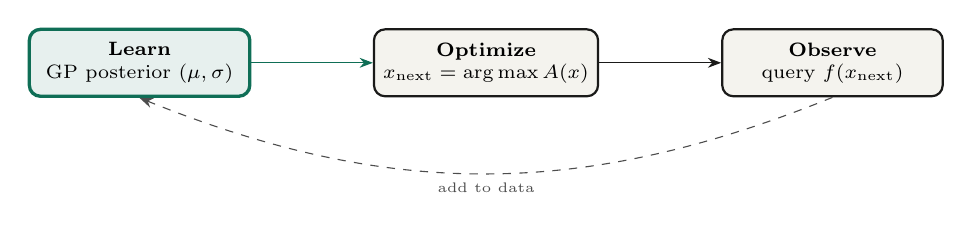
\begin{tikzpicture}[font=\scriptsize, node distance=8pt]
\node[draw=mDarkTeal, very thick, fill=mDarkTeal!10, rounded corners, minimum width=2.8cm, minimum height=0.85cm, align=center] (learn) at (0,0) {\textbf{Learn}\\ \scriptsize GP posterior $(\mu,\sigma)$};
\node[draw=mDarkBrown, thick, fill=mPaleBg, rounded corners, minimum width=2.8cm, minimum height=0.85cm, align=center] (opt) at (4.4,0) {\textbf{Optimize}\\ \scriptsize $x_{\text{next}}=\arg\max A(x)$};
\node[draw=mDarkBrown, thick, fill=mPaleBg, rounded corners, minimum width=2.8cm, minimum height=0.85cm, align=center] (obs) at (8.8,0) {\textbf{Observe}\\ \scriptsize query $f(x_{\text{next}})$};
\draw[-{Stealth}, mDarkTeal] (learn)--(opt);
\draw[-{Stealth}, mDarkBrown] (opt)--(obs);
\draw[-{Stealth}, mLightBrown, dashed] (obs.south) to[bend left=22] node[below,font=\tiny]{add to data} (learn.south);
\end{tikzpicture}
\end{center}
\medskip

\pause
Trace the lineage of each box: \emph{Learn} is Lecture 2's Bayesian update (now over a function); \emph{Optimize} is Lecture 1's optimization (now over a cheap surrogate); \emph{Observe} is the single expensive query we are trying to spend wisely. Three earlier lectures, fused into one loop.
\medskip

\pause
\begin{center}\large
This loop \emph{is} a policy: history $\to$ next action. It is the course's first taste of acting under uncertainty over time.
\end{center}
\end{frame}

%==========================================================
\section{Act 4 --- beyond, toward RL}
%==========================================================

\begin{frame}{From a function to a context --- contextual BO}
\qstrip{4}
\medskip
Often the best action depends on a \alert{context} $c$ revealed before each decision: the best price given the season, the best treatment given the patient. The policy maps context to action:
\[
\pi: c \mapsto x, \qquad x^* = \pi^*(c) = \arg\max_x f(x; c).
\]
\medskip

\pause
Now look at what we have built. A policy that, at each round, uses all past $(c, x, y)$ to choose the next $x$, maintaining a \alert{belief state} over $f$ --- and acts to maximize cumulative reward. This is precisely an \alert{MDP over the belief state}.
\medskip

\pause
\begin{center}\large
Bayesian optimization is a \alert{bandit}; contextual BO is a \alert{contextual bandit} ---
\end{center}
and the contextual bandit sits exactly between the one-shot bandit and full reinforcement learning. The only missing ingredient is \emph{state dynamics}: in BO our action doesn't change the world's state. Add that, and we have RL.
\end{frame}

\begin{frame}{The bridge --- from bandit to reinforcement learning}
\begin{center}\footnotesize\renewcommand{\arraystretch}{1.5}
\begin{tabular}{r|c|c}
 & \textbf{Single state} & \textbf{State has dynamics} \\
\hline
\textbf{non-associative}  & bandit / BO & --- \\
\hline
\textbf{associative (context)} & \cellcolor{mDarkTeal!12}contextual bandit & \cellcolor{mDarkTeal!20}\textbf{reinforcement learning} \\
\end{tabular}
\end{center}
\medskip

\pause
Reading across the row: as soon as the agent's action also \alert{changes the future state} --- not just the immediate reward --- a contextual bandit becomes a full RL problem. The explore--exploit machinery of this lecture carries over intact; what is added is the value function to account for the future an action unlocks (Lecture 7).
\medskip

\pause
{\footnotesize\textcolor{mLightBrown}{Other black-box optimizers fill the same niche --- e.g.\ CMA-ES evolves a search distribution rather than a GP --- but the BO loop is the one that most clearly prefigures the RL policy.}}
\end{frame}

%==========================================================
\section{Closing}
%==========================================================

\begin{frame}{Where we are --- Part II complete}
\vspace{2pt}
\begin{center}\footnotesize\renewcommand{\arraystretch}{1.5}
\begin{tabular}{r|c|c}
 & \textbf{Model-based} & \textbf{Data-driven} \\
\hline
\textbf{Static, single}  & optimization \;{\scriptsize Lec.\ 1 \checkmark} & Bayesian stats/net \;{\scriptsize Lec.\ 2--3 \checkmark} $\to$ \cellcolor{mDarkTeal!15}\textbf{Bayesian opt.} \;{\scriptsize Lec.\ 4 \checkmark}\\
\end{tabular}
\end{center}
\medskip

\pause
We have closed the loop: belief that chooses, observes, and updates --- an active optimizer for expensive unknowns. Two roads lead out:
\begin{itemize}\setlength\itemsep{1pt}
\item \textbf{Lectures 5--6:} what if we \alert{cannot query} $f$ live --- only a fixed dataset? Offline, data-driven design optimization (surrogate and generative).
\item \textbf{Lectures 7--10:} add \alert{state dynamics} to the loop, and the bandit becomes reinforcement learning.
\end{itemize}
\end{frame}

\begin{frame}{Closing --- the one sentence}
\vfill
\begin{center}\large
A known objective can be optimized; an \emph{unknown, expensive} one must be \alert{learned while it is optimized} ---\\[8pt]
a Gaussian process for the belief,\\[4pt]
an acquisition function to weigh learning against winning,\\[4pt]
and a loop that, quietly, is the first reinforcement learner.
\end{center}
\vfill
\pause
\footnotesize
Bayesian optimization is where modeling (Ch 1--3) becomes acting. Its explore--exploit core, its belief state, its policy-over-history --- all reappear, scaled up, the moment we let actions move the world. That move begins Part IV.
\end{frame}

\begin{frame}[standout]
Questions?
\end{frame}

%==========================================================
\appendix
%==========================================================

\begin{frame}{Backup 1 --- the GP posterior, from Gaussian conditioning}
\footnotesize
The GP posterior is one application of a single linear-algebra fact.
\medskip
\textbf{Gaussian conditioning.} If $\begin{bmatrix}Y_1\\Y_2\end{bmatrix}\sim\mathcal{N}\!\left(\begin{bmatrix}\mu_1\\\mu_2\end{bmatrix},\begin{bmatrix}\Sigma_{11}&\Sigma_{12}\\\Sigma_{21}&\Sigma_{22}\end{bmatrix}\right)$, then
\[
Y_2\mid Y_1 = y \sim \mathcal{N}\big(\mu_2 + \Sigma_{21}\Sigma_{11}^{-1}(y-\mu_1),\; \Sigma_{22}-\Sigma_{21}\Sigma_{11}^{-1}\Sigma_{12}\big).
\]
\textbf{Apply it.} Let $Y_1 = \mathbf{y}_{1:n}$ (observed, with noise variance $\sigma_\epsilon^2$ on the diagonal) and $Y_2 = f(x)$ (the value we want). Then $\Sigma_{11} = \mathbf{K}+\sigma_\epsilon^2\mathbf{I}$, $\Sigma_{21}=\mathbf{k}^\top$, $\Sigma_{22}=k(x,x)$, giving exactly
\[
\mu(x\mid\mathcal{D}) = \mathbf{k}^\top(\mathbf{K}+\sigma_\epsilon^2\mathbf{I})^{-1}\mathbf{y}, \qquad \sigma^2(x\mid\mathcal{D}) = k(x,x)-\mathbf{k}^\top(\mathbf{K}+\sigma_\epsilon^2\mathbf{I})^{-1}\mathbf{k}. \quad\blacksquare
\]
The mean is a kernel-weighted average of observed $y$'s; the variance shrinks near data and returns to the prior $k(x,x)$ far from it.
\end{frame}

\begin{frame}{Backup 2 --- kernels and hyperparameters}
\footnotesize
The kernel encodes assumed structure; its hyperparameters are learned from data.
\medskip
\textbf{Common kernels.}
\begin{itemize}\setlength\itemsep{1pt}
\item \textbf{Squared exponential (SE):} $k(x,x')=\sigma_0^2\exp(-\tfrac{1}{2}\|x-x'\|^2/\lambda^2)$ --- very smooth (infinitely differentiable); $\lambda$ is the length scale.
\item \textbf{Mat\'ern:} rougher, finitely-differentiable sample paths --- often more realistic for physical functions.
\item \textbf{ARD:} a separate length scale $\lambda_d$ per input dimension; large $\lambda_d$ $\Rightarrow$ dimension $d$ is irrelevant (automatic relevance determination).
\end{itemize}
\medskip
\textbf{Fitting hyperparameters $\theta=(\sigma_\epsilon,\sigma_0,\lambda)$.} Maximize the marginal log-likelihood of the data:
\[
\theta^* = \arg\max_\theta\Big[-\tfrac12\mathbf{y}^\top(\mathbf{K}_\theta+\sigma_\epsilon^2\mathbf{I})^{-1}\mathbf{y} - \tfrac12\log|\mathbf{K}_\theta+\sigma_\epsilon^2\mathbf{I}| - \tfrac{n}{2}\log 2\pi\Big].
\]
The first term rewards fitting the data; the second penalizes model complexity --- an automatic Occam balance, itself an optimization (Lecture 1) inside the loop.
\end{frame}

\begin{frame}{Backup 3 --- Expected Improvement, in closed form}
\footnotesize
With posterior $f(x)\sim\mathcal{N}(\mu,\sigma^2)$ and current best $f^{\max}$, define the improvement $I = \max(0, f(x)-f^{\max})$. Its expectation has a closed form:
\[
\mathrm{EI}(x) = (\mu - f^{\max})\,\Phi(z) + \sigma\,\phi(z), \qquad z = \frac{\mu - f^{\max}}{\sigma},
\]
where $\Phi,\phi$ are the standard normal CDF and PDF.
\medskip
\textbf{Reading the two terms.}
\begin{itemize}\setlength\itemsep{1pt}
\item $(\mu-f^{\max})\Phi(z)$ --- the \alert{exploit} term: large where the mean already beats the best.
\item $\sigma\,\phi(z)$ --- the \alert{explore} term: large where uncertainty is high, even if the mean is unremarkable.
\end{itemize}
\medskip
EI needs \emph{no} tuning parameter to balance the two --- the trade-off falls out of the Gaussian. (UCB's $\mu+\kappa\sigma$ exposes the same balance through an explicit knob $\kappa$.) Maximizing $\mathrm{EI}(x)$ is the cheap inner optimization that selects each expensive query.
\end{frame}

\end{document}
